 \documentclass[t, xcolor=table]{beamer}
%\documentclass[c]{beamer}
\listfiles

\newcommand{\putat}[3]{\begin{picture}(0,0)(0,0)\put(#1,#2){#3}\end{picture}}
\newcommand*{\xMin}{-6}%
\newcommand*{\xMax}{6}%
\newcommand*{\yMin}{-6}%
\newcommand*{\yMax}{5}%
\setbeamertemplate{section in toc}[sections numbered]
\setbeamertemplate{subsection in toc}[subsections numbered]

\defbeamertemplate{subsubsection in toc}{subsubsections numbered}
{\leavevmode\leftskip=3em%
 \rlap{\hskip-3em\inserttocsectionnumber.\inserttocsubsectionnumber.\inserttocsubsubsectionnumber}%
 \inserttocsubsubsection\par}



\mode<presentation>
{
  \usetheme[usefoot,english,cmyk,titlepage0]{KIT}
% \usetheme[usefoot]{KIT}
% \usetheme{KIT}

%%  \usefonttheme{structurebold}

  \setbeamercovered{transparent}

  %\setbeamertemplate{enumerate items}[circle]
  \setbeamertemplate{enumerate items}[ball]
%  \setbeamerfont{section in toc}{color=black}
  \setbeamercolor{section number projected}{bg=black,fg=yellow}
  \setbeamertemplate{subsection in toc}[subsubsections numbered]

}
\usepackage{tabularx}
\usepackage{pdfpages}
\usepackage{caption}
\usepackage{pbox}
\usepackage{multirow}
\usepackage{babel}
\usepackage{feynmp-auto}
\usetikzlibrary{calc}
\date{09.07.2018}
%\DateText

\newlength{\Ku}
\setlength{\Ku}{1.43375pt}

\usepackage[latin1]{inputenc}
\usepackage[TS1,T1]{fontenc}
\usepackage{array}
\usepackage{multicol}
\usepackage[makeroom]{cancel}
\usepackage{subfigure}
\usepackage{xspace}
%\usenavigationsymbols
%\usenavigationsymbols[sfHhdb]
%\usenavigationsymbols[sfhHb]
\newcommand{\verysmall}{\fontsize{6pt}{8.6pt}\selectfont}
\usepackage{siunitx}


\DeclareSIUnit\clight{\ensuremath{c}}
\DeclareSIUnit[per-mode=symbol]\GeVc{\GeV\per\clight}
\DeclareSIUnit[per-mode=symbol]\GeVcc{\GeV\per\clight\squared}
\DeclareSIUnit\fb{\femto\barn}
\DeclareSIUnit\invfb{\per\femto\barn}

\newenvironment<>{neutralblock}[1]{%
  \begin{actionenv}#2%
      \def\insertblocktitle{#1}%
      \par%
      \mode<presentation>{%
        \setbeamercolor{block title}{fg=white,bg=gray!70!black}
       \setbeamercolor{block body}{fg=black,bg=gray!50}
       \setbeamercolor{itemize item}{fg=white}
       \setbeamertemplate{itemize item}[triangle]
     }%
      \usebeamertemplate{block begin}}
    {\par\usebeamertemplate{block end}\end{actionenv}}

\newenvironment<>{redblock}[1]{%
  \begin{actionenv}#2%
      \def\insertblocktitle{#1}%
      \par%
      \mode<presentation>{%
        \setbeamercolor{block title}{fg=white,bg=red!70!black}
       \setbeamercolor{block body}{fg=black,bg=red!30}
       \setbeamercolor{itemize item}{fg=white}
       \setbeamertemplate{itemize item}[triangle]
     }%
      \usebeamertemplate{block begin}}
    {\par\usebeamertemplate{block end}\end{actionenv}}

\newenvironment<>{blueblock}[1]{%
  \begin{actionenv}#2%
      \def\insertblocktitle{#1}%
      \par%
      \mode<presentation>{%
        \setbeamercolor{block title}{fg=white,bg=blue!70!black}
       \setbeamercolor{block body}{fg=black,bg=blue!30!white!80}
       \setbeamercolor{itemize item}{fg=white}
       \setbeamertemplate{itemize item}[triangle]
     }%
      \usebeamertemplate{block begin}}
    {\par\usebeamertemplate{block end}\end{actionenv}}

\newenvironment<>{greenblock}[1]{%
  \begin{actionenv}#2%
      \def\insertblocktitle{#1}%
      \par%
      \mode<presentation>{%
        \setbeamercolor{block title}{fg=white,bg=green!70!black}
       \setbeamercolor{block body}{fg=black,bg=green!50}
       \setbeamercolor{itemize item}{fg=white}
       \setbeamertemplate{itemize item}[triangle]
     }%
      \usebeamertemplate{block begin}}
    {\par\usebeamertemplate{block end}\end{actionenv}}

\title[]{Modeling and Simulation of Load Balancing Strategies for Computing in High Energy Physics}
\subtitle{Karlsruhe Institute of Technology (KIT)}

\subtitle[Ren\'e Caspart]{\underline{\smash{Ren\'e Caspart}}, Patrick Firnkes, Manuel Giffels, Anne Koziolek, G\"unter Quast, Ralf Reussner}

\AuthorTitleSep{\relax}

\institute[]{KARLSRUHE INSTITUTE OF TECHNOLOGY (KIT)}

\TitleImage[width=\titleimagewd]{Bilder/KIT-Titel}

\newlength{\tmplen}

\begin{document}


%%%%%%%%%%%%%%%%%%%%%%%%%%%%%%%%%%%%%%%%%%%%%%%%%%%%%%%%%%%%%%%%%%%%%%%%%%%%%%%%%%%%%%%%%%%%%%%%%%%%%%%%%%%%%%%%%%%%%%%%%%%%%%%%%%%%%%%%%%%%%%
\begin{frame}
  \maketitle
\end{frame}

%%%%%%%%%%%%%%%%%%%%%%%%%%%%%%%%%%%%%%%%%%%%%%%%%%%%%%%%%%%%%%%%%%%%%%%%%%%%%%%%%%%%%%%%%%%%%%%%%%%%%%%%%%%%%%%%%%%%%%%%%%%%%%%%%%%%%%%%%%%%%%
\AtBeginSection[]
{
\begin{frame}
\frametitle{Table of Contents}
\tableofcontents[currentsection,%currentsubsection, 
%    hideothersubsections, 
    sectionstyle=show/shaded,
    subsectionstyle=hide/hide,
]
\end{frame}
}

%%%%%%%%%%%%%%%%%%%%%%%%%%%%%%%%%%%%%%%%%%%%%%%%%%%%%%%%%%%%%%%%%%%%%%%%%%%%%%%%%%%%%%%%%%%%%%%%%%%%%%%%%%%%%%%%%%%%%%%%%%%%%%%%%%%%%%%%%%%%%%

\section*{Motivation}
\begin{frame}
    \frametitle{Motivation}
    \begin{columns}
        \begin{column}{0.45\textwidth}
            \begin{itemize}
                \item 1
                \item 2
            \end{itemize}
        \end{column}
        \hfill
        \begin{column}{0.45\textwidth}
            \begin{itemize}
                \item 3
                \item 4
            \end{itemize}
        \end{column}
    \end{columns}
\end{frame}



\section*{Palladio Simulator}
\begin{frame}
\frametitle{Palladio Simulator}
\begin{columns}
	\begin{column}{0.45\textwidth}
		\begin{itemize}
			 \setlength\itemsep{1em}
			\item Model driven software architecture simulator
			\item Developed at KIT, FZI and University of Paderborn
			\item Enables performance predictions \\ {\scriptsize (Reussner et al., 2016)}
		\end{itemize}
		\putat{50}{-45}{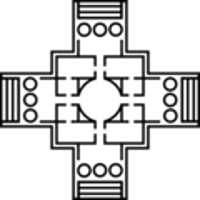
\includegraphics[scale=0.5]{Bilder/palladio-logo}}
		\putat{50}{-55}{{\scriptsize Palladio Logo}}
		\putat{35}{-65}{{\scriptsize (http://palladio-simulator.com)}}
	\end{column}
	\hfill
	\begin{column}{0.45\textwidth}
		\begin{itemize}
			 \setlength\itemsep{1em}
			\item Extended for simulation of Cloud Computing/HPC
			\begin{itemize}
				\item Architectural Templates \\ {\scriptsize (Lehrig \& Becker, 2016)}
				\item SimuLizar \\ {\scriptsize (Becker et al., 2013)}

			\end{itemize}
			\item Successfully used for optimizing cloud infrastructure \\ {\scriptsize (Ostberg et al., 2014)}

		\end{itemize}
	\end{column}
\end{columns}
\end{frame}

\note[itemize]{

\item Palladio should be used to evaluate different load balancing strategies or other design decisions (like infrastructure improvements).

\item Architectural Templates: Enables one to efficiently model large systems (E.g. instead of modeling 1000 servers manuelly, model one server and architectural templates duplicates this server 1000 times).

\item SimuLizar: Simulation engine that enables one to model self adpating systems.

\item Palladio/SimuLizar successfully used to optimize cloud infrastructure as part of the CACTOS project
}


\section*{Model}
\begin{frame}
\frametitle{Model}
\begin{columns}
	\begin{column}{0.45\textwidth}
		\begin{itemize}
		\setlength\itemsep{1em}
			\item Model each kind of computing job with its resource requirements
				\begin{itemize}
					\item CPU \& I/O
					\item Required job slots
					\item Number of events
				\end{itemize}
			\item Model each type of computing node
				\begin{itemize}
					\item Number and processing speed of cores
					\item Processing speed of I/O
					\item Number of job slots
					\item Number of instances of node
				\end{itemize}
			\end{itemize}
	\end{column}
	\hfill
	\begin{column}{0.45\textwidth}
		\begin{itemize}
		\setlength\itemsep{1em}
		\item Model load balancing strategy
			\begin{itemize}
				\item First fit search based on available job slots
				\item Easily modifiable to evaluate new strategies
			\end{itemize}
		
		\item Model high load on system
			\begin{itemize}
				\item Closed workload
				\item Enough jobs to guarantee that systems never idles
				\item Each job type has configurable share of load
			\end{itemize}
		\end{itemize}
	\end{column}
\end{columns}
\end{frame}

\note[itemize]{
	\item Different Models of the system are created, on for the resource environment, the assembly (how components work togehter), the usage, the allocation and the component behaviour (e.g. required resources).
	
	\item Required Resources are probability distributions
	\item Jobs block and wait for free slots if not enough job slots are available on working node.
		
	\item Closed workload: there are always 2500 jobs being processed or waiting to be processed.
}


\begin{frame}
\frametitle{Model}
\begin{columns}
	\begin{column}{0.45\textwidth}
			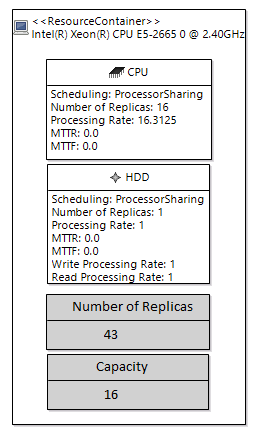
\includegraphics[scale=0.5]{Bilder/model-container}
	\end{column}

	\begin{column}{0.45\textwidth}
			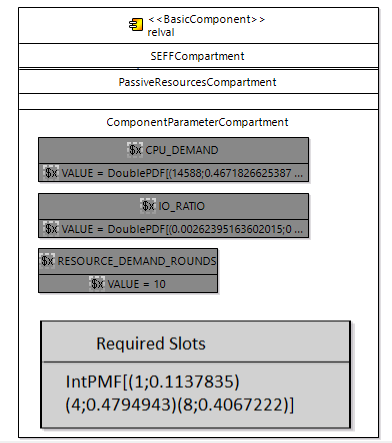
\includegraphics[scale=0.5]{Bilder/component}
	\end{column}
\end{columns}
\end{frame}

\section*{Results}
\begin{frame}
\frametitle{Results}
			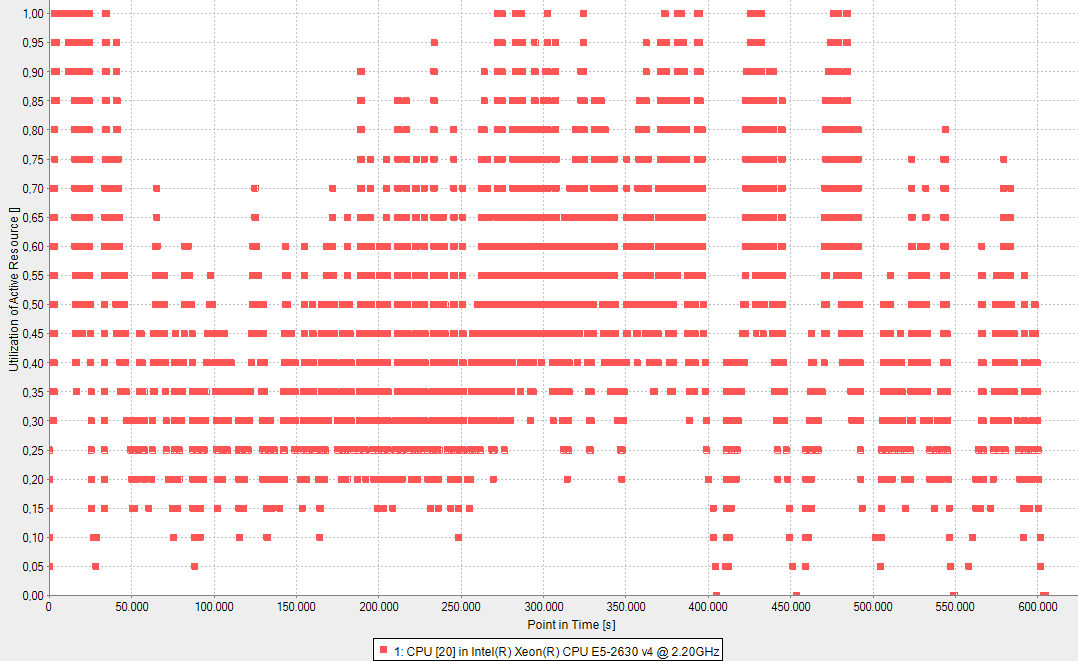
\includegraphics[scale=0.42]{Bilder/utilization}
\end{frame}

\note[itemize]{
	\item Required time to simulate one week is 12-13min.
	\item Validated with throughput and share of completed jobs per type
	\item Not yet validated with measured utilization.
}

\section*{Outlook}
\begin{frame}
\frametitle{Outlook}
\begin{columns}
	\begin{column}{0.45\textwidth}
		\begin{itemize}
			\item 1
			\item 2
		\end{itemize}
	\end{column}
	\hfill
	\begin{column}{0.45\textwidth}
		\begin{itemize}
			\item 3
			\item 4
		\end{itemize}
	\end{column}
\end{columns}
\end{frame}
\end{document}
